\section{Задача протекания}

\subsection{Постановка задачи}
Задана область $$\Omega = \Omega_{01} \cup \Omega_{02} \cup \Omega_{11} \cup \Omega_{12} \cup \Omega_{10} \cup \Omega_{10} \cup \Omega_{20} $$

Неизвестные функции: плотность $\rho$ и вектор скорости $\vec{u}$ являются функциями переменных Эйлера $(t, x) \in Q = [0, T] \times \Omega$.

Граничные условия для неизвестного решения: 
$$
	\rho \big|_{\Gamma-} = \rho_\gamma   \,, \quad
	u_1 \big|_{\Gamma-} = w              \,, \quad
	\deriv{u_1}{x} \big|_{\Gamma+} = 0
$$
На оставшейся границе компоненты скорости равны нулю, а функция плотности считается неизвестной.

\begin{figure}[h!] \centering
	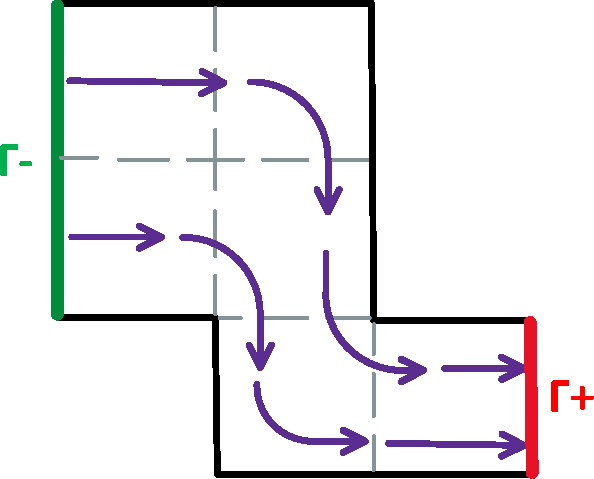
\includegraphics[scale=0.6]{area_2.pdf}
	\captionof{figure}{Заданная область}
\end{figure}


\subsection{Численные эксперименты}
Будем рассматривать зависимости $ p(\rho) = C \rho, \; C \in \{1, 10\} $, а также параметры  $\mu \in \{0.1, 0.01, 0.001\}$, $\rho_\gamma \in \{1, 10\}$. Если предыдущее состояние газа не отличается от текущего на $\epsilon = 10^{-3}$, то останавливаем расчёт. При фиксированных $\tau$, $h_1 = h_2 = h$ будем исследовать момент завершения программы.  \\

%Значение времени, помеченное $*$ означает, что схема разошлась в этот момент времени. \\

Будут приведены графики на рассматриваемой области, иллюстрирующие изменение плотности и векторов скорости от момента времени.\\

Для решения системы $Ax = b$ использовался метод $BiCGSTab$ + $ILUT$ предобусловливатель из библиотеки Eigen (см. \cite{Eigen}) с параметрами $eps = 10^{-8}$, $iter = 2000$.

\newpage

\subsection{$C = 1$, $\mu = 0.10$, $w = 0.5$, $\rho_\gamma = 1$, $\tau = 0.010$, $h = 0.050$}

\begin{figure}[h!] \centering 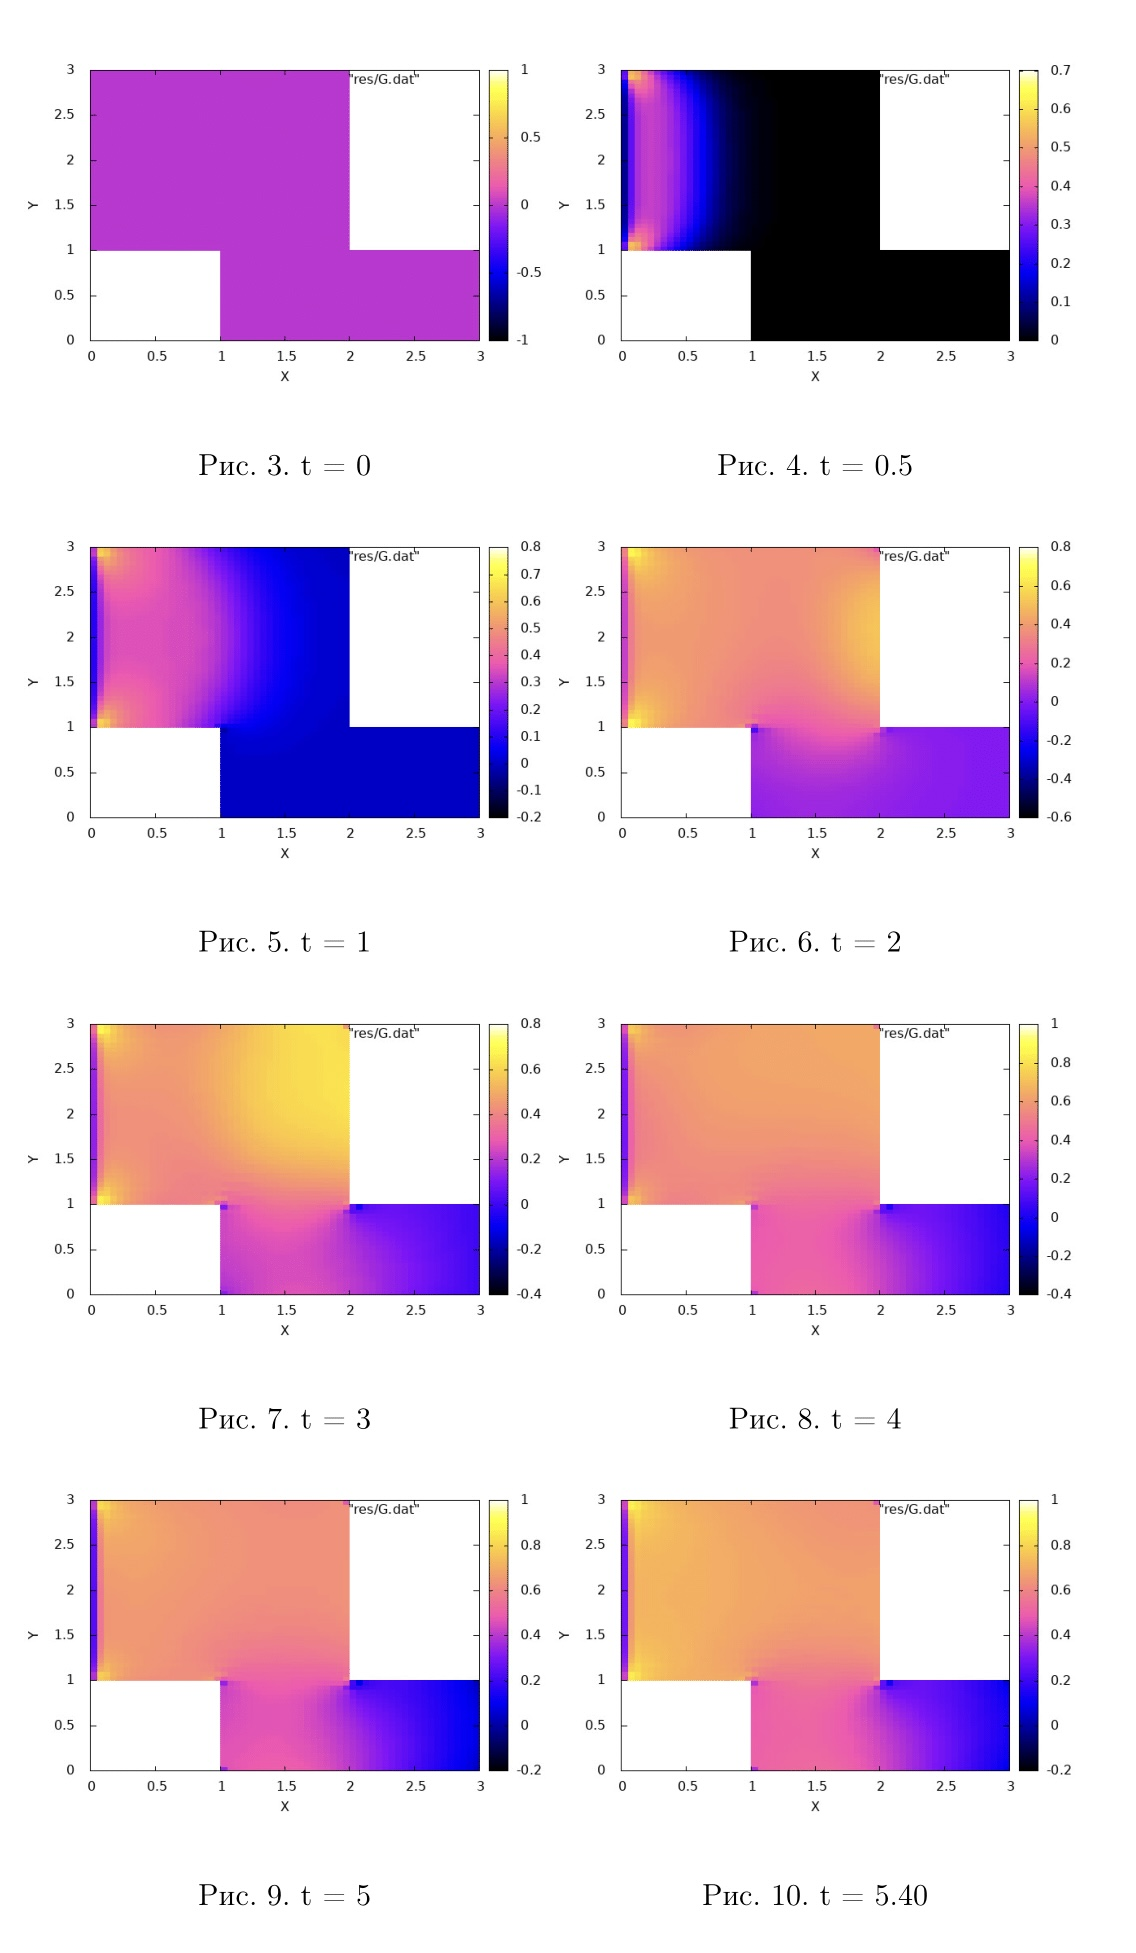
\includegraphics[scale=0.9]{tabulars-19.png} \end{figure} \newpage
\begin{figure}[h!] \centering 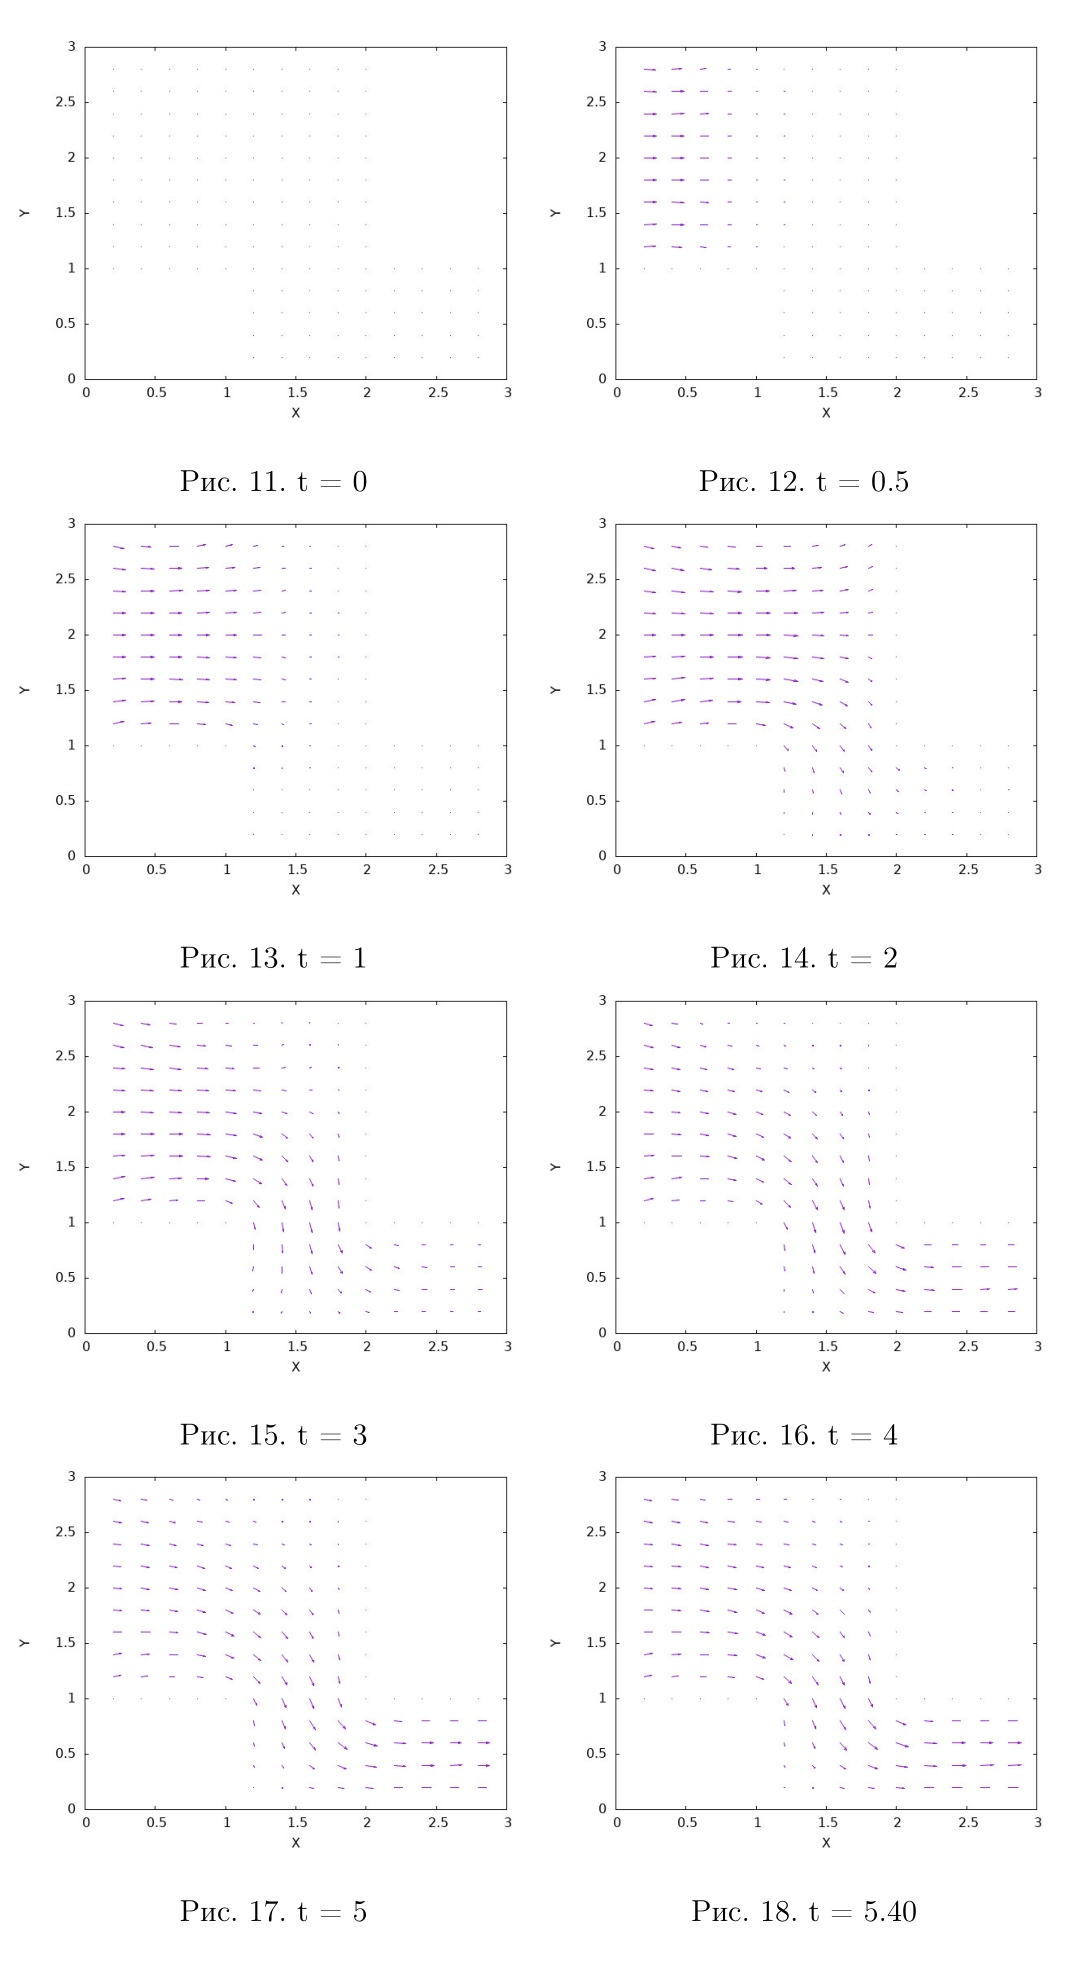
\includegraphics[scale=0.9]{tabulars-20.png} \end{figure} \newpage

\subsection{$C = 1$, $\mu = 0.01$, $w = 0.5$, $\rho_\gamma = 1$, $\tau = 0.005$, $h = 0.025$}
\begin{figure}[h!] \centering 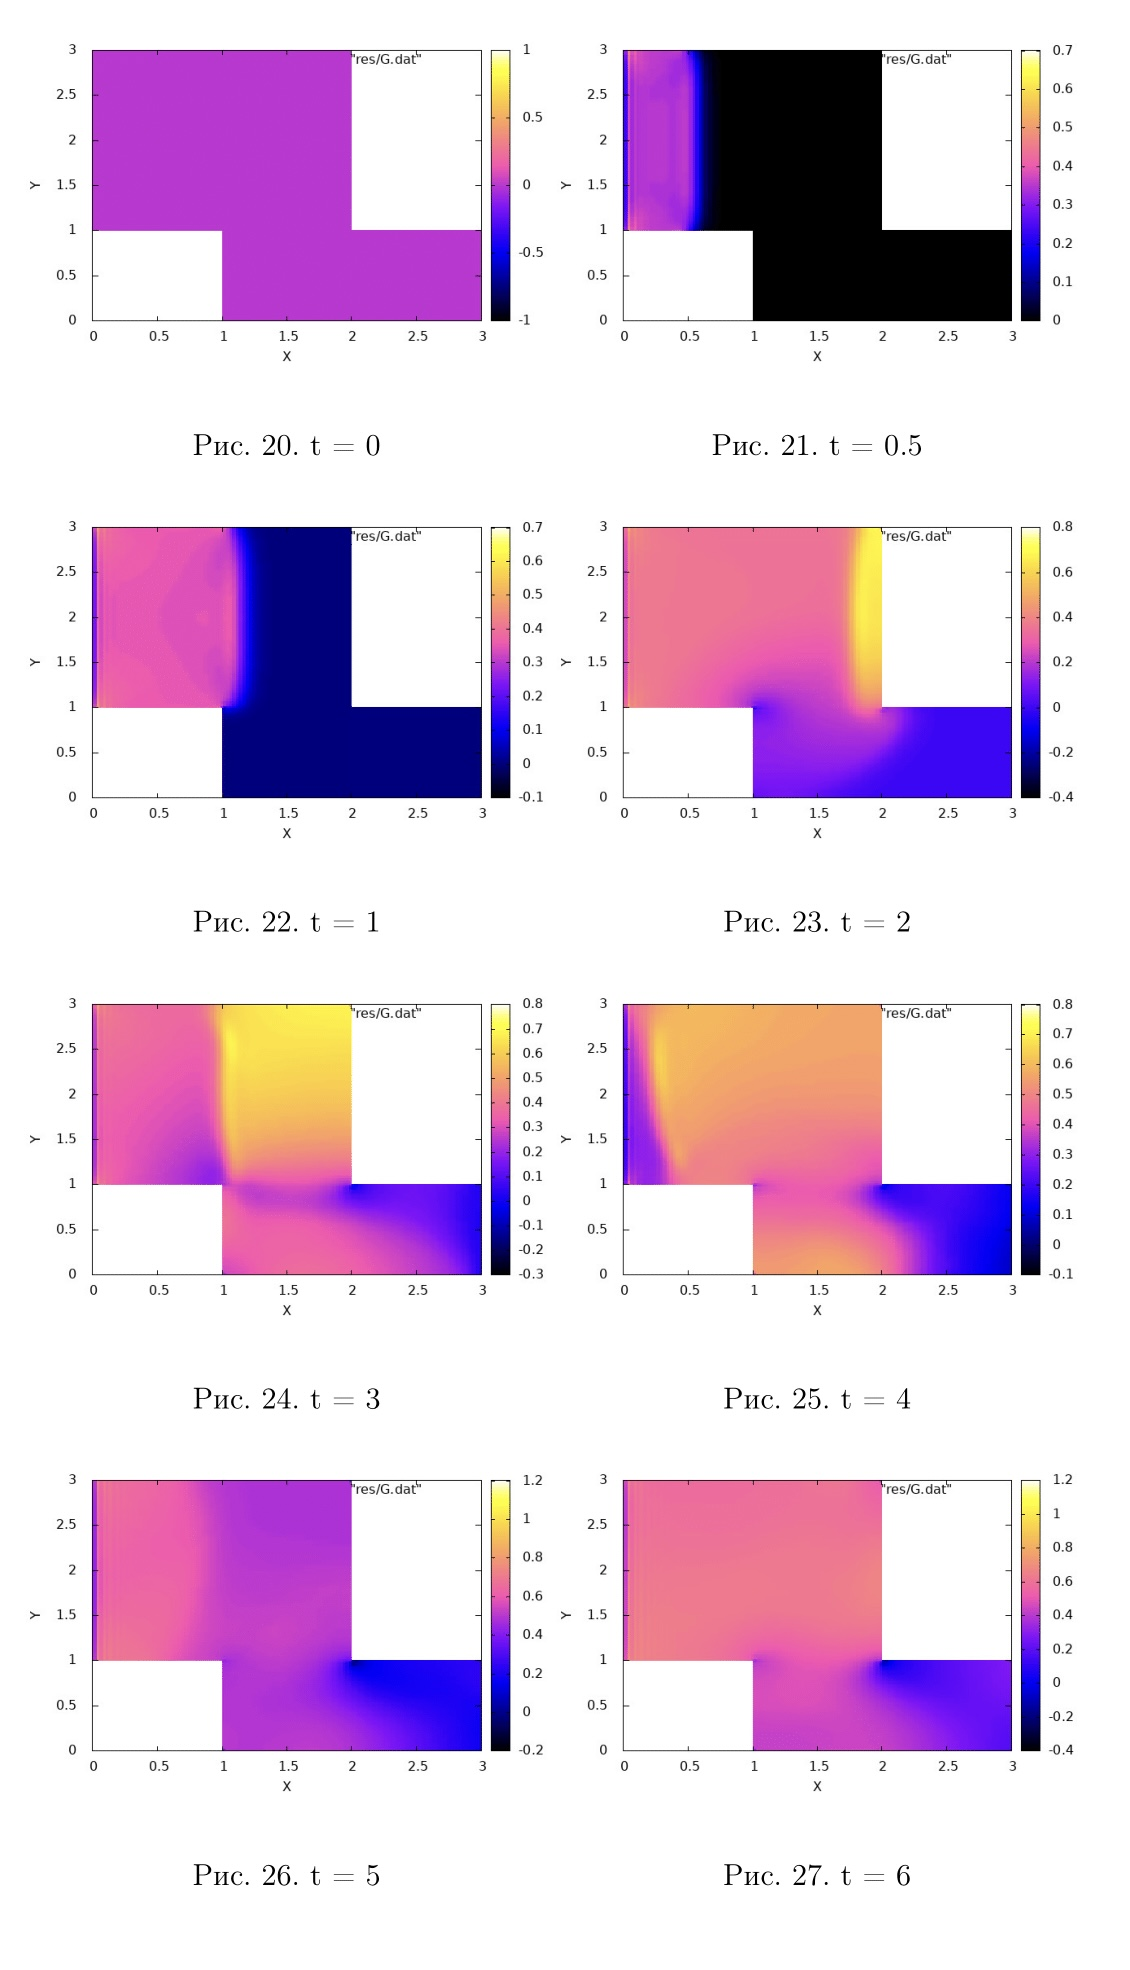
\includegraphics[scale=0.9]{tabulars-23.png} \end{figure} \newpage
\begin{figure}[h!] \centering 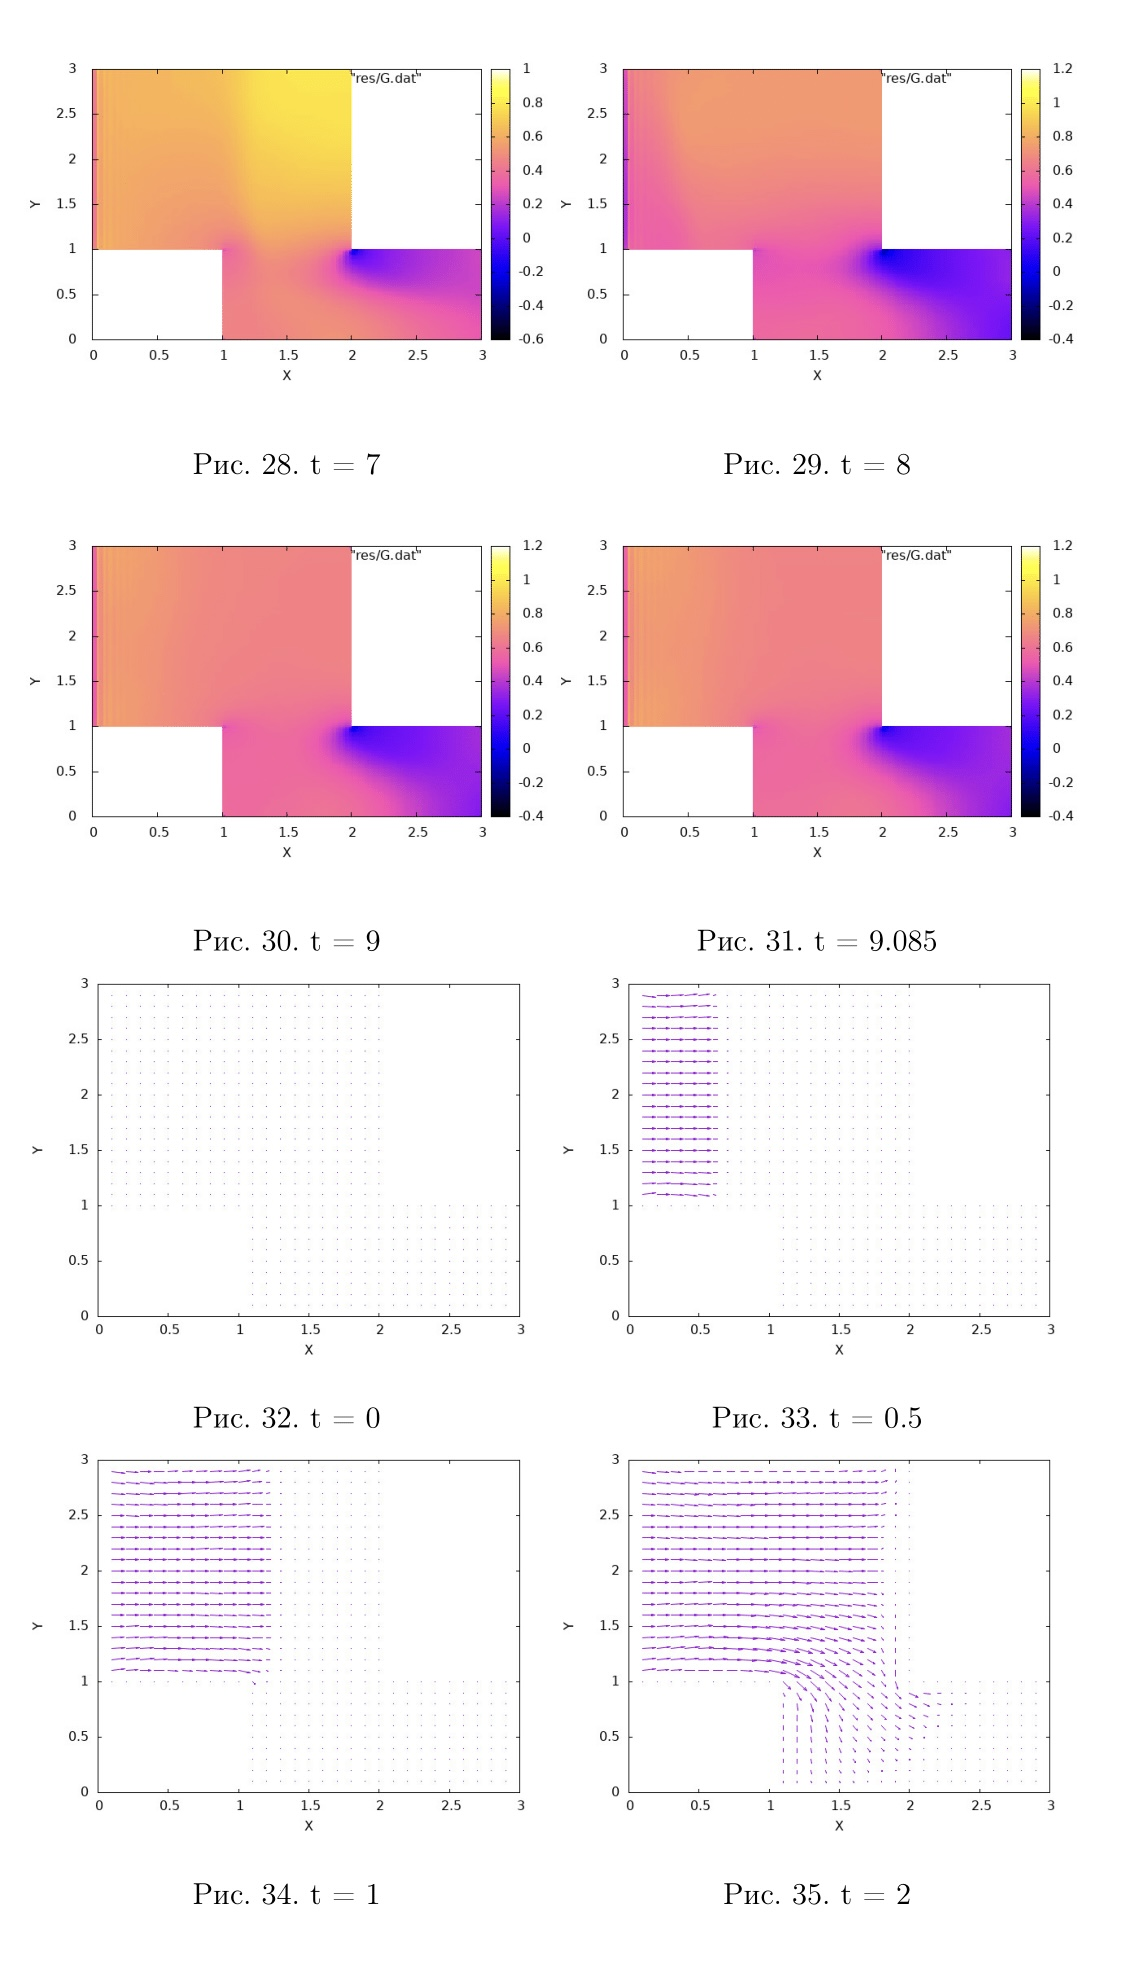
\includegraphics[scale=0.9]{tabulars-24.png} \end{figure} \newpage
\begin{figure}[h!] \centering 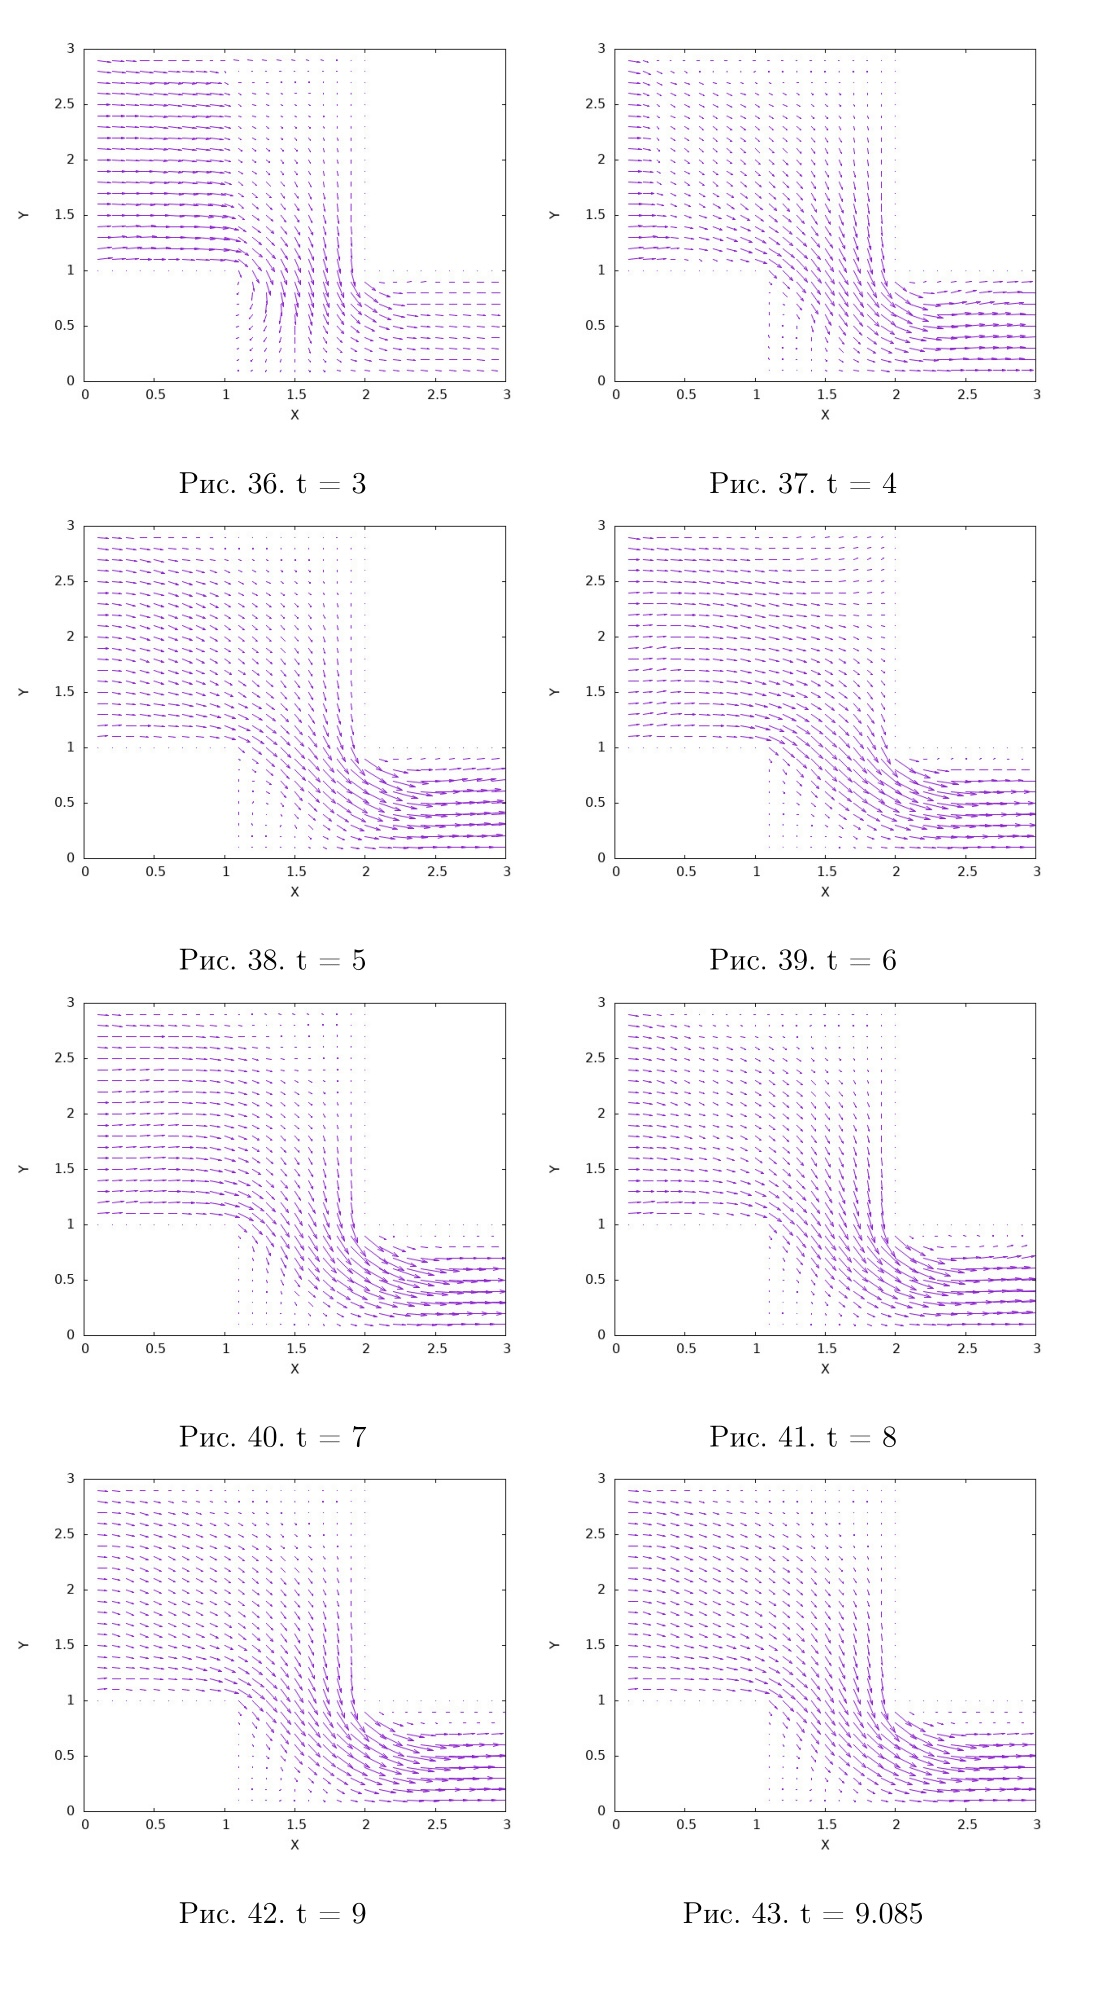
\includegraphics[scale=0.9]{tabulars-25.png} \end{figure} \newpage

\newpage

%\begin{table}[H]
\centering
\begin{tabular}{|c|c|c|c|c|}
\hline
\diagTH & $10^{-1}$ & $10^{-2}$ & $10^{-3}$ & $10^{-4}$ \\
\hline
 & \texttt{1.181652e+01} & \texttt{1.443212e+00} & \texttt{1.443281e+00} & \texttt{1.443604e+00} \\
$10^{-1}$ & \texttt{4.893319e+00} & \texttt{8.042684e-01} & \texttt{8.003429e-01} & \texttt{8.002513e-01} \\
 & \texttt{3.968220e+01} & \texttt{7.933857e+00} & \texttt{7.912020e+00} & \texttt{7.926450e+00} \\
\hline
 & \texttt{6.248864e+01} & \texttt{1.766651e-01} & \texttt{1.708897e-01} & \texttt{1.708306e-01} \\
$10^{-2}$ & \texttt{1.900438e+01} & \texttt{9.811932e-02} & \texttt{9.445940e-02} & \texttt{9.442351e-02} \\
 & \texttt{1.708589e+02} & \texttt{7.879295e-01} & \texttt{7.587913e-01} & \texttt{7.584994e-01} \\
\hline
 & \texttt{7.120057e+00} & \texttt{2.252087e-02} & \texttt{1.756171e-02} & \texttt{1.751225e-02} \\
$10^{-3}$ & \texttt{1.926111e+00} & \texttt{1.232548e-02} & \texttt{9.001833e-03} & \texttt{8.971483e-03} \\
 & \texttt{2.143837e+01} & \texttt{1.042810e-01} & \texttt{8.186950e-02} & \texttt{8.180130e-02} \\
\hline
 & \texttt{2.155197e+00} & \texttt{6.803025e-03} & \texttt{1.804239e-03} & \texttt{1.755320e-03} \\
$10^{-4}$ & \texttt{1.278056e+00} & \texttt{4.675248e-03} & \texttt{9.227605e-04} & \texttt{8.926073e-04} \\
 & \texttt{1.193935e+01} & \texttt{3.956212e-02} & \texttt{8.415822e-03} & \texttt{8.227393e-03} \\
\hline
\end{tabular}
\caption{Ошибки для схемы \texttt{1} при $C = 1$, $\gamma = 1$ и~$\mu = 0.1$.}
\end{table}

\begin{table}[H]
\centering
\begin{tabular}{|c|c|c|c|c|}
\hline
\diagTH & $10^{-1}$ & $10^{-2}$ & $10^{-3}$ & $10^{-4}$ \\
\hline
 & \texttt{3.222515e+00} & \texttt{1.462851e-01} & \texttt{1.440101e-01} & \texttt{1.439917e-01} \\
$10^{-1}$ & \texttt{1.120161e+00} & \texttt{6.801977e-02} & \texttt{6.715263e-02} & \texttt{6.714411e-02} \\
 & \texttt{1.339440e+01} & \texttt{8.824962e-01} & \texttt{9.035803e-01} & \texttt{9.042429e-01} \\
\hline
 & \texttt{5.048784e+01} & \texttt{2.294542e-02} & \texttt{2.236461e-02} & \texttt{2.235894e-02} \\
$10^{-2}$ & \texttt{1.562821e+01} & \texttt{1.154502e-02} & \texttt{1.111025e-02} & \texttt{1.110629e-02} \\
 & \texttt{9.405579e+01} & \texttt{1.030876e-01} & \texttt{9.997687e-02} & \texttt{1.001472e-01} \\
\hline
 & \texttt{9.549526e+02} & \texttt{3.727700e-03} & \texttt{2.617173e-03} & \texttt{2.610631e-03} \\
$10^{-3}$ & \texttt{4.195816e+02} & \texttt{1.869996e-03} & \texttt{1.296306e-03} & \texttt{1.292612e-03} \\
 & \texttt{1.360581e+03} & \texttt{2.412181e-02} & \texttt{1.041279e-02} & \texttt{1.037825e-02} \\
\hline
 & \texttt{8.625099e+02} & \texttt{3.212226e-03} & \texttt{2.719209e-04} & \texttt{2.652392e-04} \\
$10^{-4}$ & \texttt{4.645395e+02} & \texttt{9.819210e-04} & \texttt{1.352273e-04} & \texttt{1.313576e-04} \\
 & \texttt{1.326580e+03} & \texttt{1.802712e-02} & \texttt{1.133119e-03} & \texttt{1.042953e-03} \\
\hline
\end{tabular}
\caption{Ошибки для схемы \texttt{1} при $C = 10$, $\gamma = 1$ и~$\mu = 0.1$.}
\end{table}

\begin{table}[H]
\centering
\begin{tabular}{|c|c|c|c|c|}
\hline
\diagTH & $10^{-1}$ & $10^{-2}$ & $10^{-3}$ & $10^{-4}$ \\
\hline
 & \texttt{4.851430e+04} & \texttt{1.183144e-01} & \texttt{1.022894e-02} & \texttt{1.020089e-02} \\
$10^{-1}$ & \texttt{2.208050e+04} & \texttt{1.769615e-02} & \texttt{6.105316e-03} & \texttt{6.099189e-03} \\
 & \texttt{3.103531e+05} & \texttt{1.126021e+00} & \texttt{6.339364e-02} & \texttt{6.348438e-02} \\
\hline
 & \texttt{2.537852e+03} & \texttt{4.145018e-03} & \texttt{2.241746e-03} & \texttt{2.239338e-03} \\
$10^{-2}$ & \texttt{1.606647e+03} & \texttt{1.611664e-03} & \texttt{1.183370e-03} & \texttt{1.183675e-03} \\
 & \texttt{1.895135e+04} & \texttt{2.015021e-02} & \texttt{4.378571e-03} & \texttt{4.334379e-03} \\
\hline
 & \texttt{1.434099e+02} & \texttt{3.399383e-03} & \texttt{2.303365e-04} & \texttt{2.279940e-04} \\
$10^{-3}$ & \texttt{1.111249e+02} & \texttt{1.130865e-03} & \texttt{1.205005e-04} & \texttt{1.208826e-04} \\
 & \texttt{2.821377e+02} & \texttt{1.889347e-02} & \texttt{4.640649e-04} & \texttt{4.105267e-04} \\
\hline
 & \texttt{1.704815e+04} & \texttt{3.402526e-03} & \texttt{4.171373e-05} & \texttt{2.199472e-05} \\
$10^{-4}$ & \texttt{1.281007e+04} & \texttt{1.142852e-03} & \texttt{1.560524e-05} & \texttt{1.165764e-05} \\
 & \texttt{3.882601e+04} & \texttt{1.900494e-02} & \texttt{1.948088e-04} & \texttt{3.916520e-05} \\
\hline
\end{tabular}
\caption{Ошибки для схемы \texttt{1} при $C = 100$, $\gamma = 1$ и~$\mu = 0.1$.}
\end{table}

\begin{table}[H]
\centering
\begin{tabular}{|c|c|c|c|c|}
\hline
\diagTH & $10^{-1}$ & $10^{-2}$ & $10^{-3}$ & $10^{-4}$ \\
\hline
 & \texttt{9.118165e+00} & \texttt{1.153563e+00} & \texttt{1.162321e+00} & \texttt{1.162278e+00} \\
$10^{-1}$ & \texttt{3.344701e+00} & \texttt{6.000072e-01} & \texttt{5.989285e-01} & \texttt{5.990541e-01} \\
 & \texttt{3.390989e+01} & \texttt{6.012765e+00} & \texttt{5.659256e+00} & \texttt{5.685288e+00} \\
\hline
 & \texttt{8.146566e+00} & \texttt{9.039186e-02} & \texttt{8.840905e-02} & \texttt{8.838949e-02} \\
$10^{-2}$ & \texttt{5.449893e+00} & \texttt{5.340469e-02} & \texttt{5.216930e-02} & \texttt{5.215748e-02} \\
 & \texttt{3.567165e+01} & \texttt{4.388565e-01} & \texttt{4.531820e-01} & \texttt{4.561369e-01} \\
\hline
 & \texttt{3.864207e+00} & \texttt{1.062531e-02} & \texttt{8.764154e-03} & \texttt{8.747440e-03} \\
$10^{-3}$ & \texttt{1.116353e+00} & \texttt{6.322317e-03} & \texttt{4.838855e-03} & \texttt{4.828481e-03} \\
 & \texttt{1.053306e+01} & \texttt{4.526193e-02} & \texttt{4.443798e-02} & \texttt{4.485572e-02} \\
\hline
 & \texttt{4.602507e+00} & \texttt{7.991192e-03} & \texttt{8.912093e-04} & \texttt{8.744621e-04} \\
$10^{-4}$ & \texttt{1.249849e+00} & \texttt{2.789505e-03} & \texttt{4.899526e-04} & \texttt{4.791004e-04} \\
 & \texttt{1.250676e+01} & \texttt{2.929977e-02} & \texttt{4.359942e-03} & \texttt{4.469110e-03} \\
\hline
\end{tabular}
\caption{Ошибки для схемы \texttt{1} при $C = 1$, $\gamma = 1.4$ и~$\mu = 0.1$.}
\end{table}

\begin{table}[H]
\centering
\begin{tabular}{|c|c|c|c|c|}
\hline
\diagTH & $10^{-1}$ & $10^{-2}$ & $10^{-3}$ & $10^{-4}$ \\
\hline
 & \texttt{4.564166e+00} & \texttt{9.494955e-01} & \texttt{9.486571e-01} & \texttt{9.486554e-01} \\
$10^{-1}$
 & \texttt{1.573963e+00} & \texttt{5.196175e-01} & \texttt{5.187592e-01} & \texttt{5.187529e-01} \\
 & \texttt{1.560271e+01} & \texttt{5.156837e+00} & \texttt{5.054622e+00} & \texttt{5.063952e+00} \\
\hline
 & \texttt{4.794683e+01} & \texttt{1.792192e-01} & \texttt{1.776189e-01} & \texttt{1.776132e-01} \\
$10^{-2}$
 & \texttt{1.094421e+01} & \texttt{8.201671e-02} & \texttt{8.096468e-02} & \texttt{8.095492e-02} \\
 & \texttt{1.408516e+02} & \texttt{1.382530e+00} & \texttt{1.425657e+00} & \texttt{1.431199e+00} \\
\hline
 & \texttt{1.167069e+04} & \texttt{2.340101e-02} & \texttt{2.252434e-02} & \texttt{2.251531e-02} \\
$10^{-3}$
 & \texttt{5.143610e+03} & \texttt{1.035069e-02} & \texttt{8.646357e-03} & \texttt{8.636329e-03} \\
 & \texttt{1.591441e+04} & \texttt{1.650773e-01} & \texttt{1.838053e-01} & \texttt{1.841455e-01} \\
\hline
 & \texttt{3.367458e+04} & \texttt{5.953102e-03} & \texttt{2.323615e-03} & \texttt{2.314594e-03} \\
$10^{-4}$
 & \texttt{1.547585e+04} & \texttt{4.247154e-03} & \texttt{8.816500e-04} & \texttt{8.710264e-04} \\
 & \texttt{5.749273e+04} & \texttt{4.241223e-02} & \texttt{1.887922e-02} & \texttt{1.910149e-02} \\
\hline
\end{tabular}
\caption{Ошибки для схемы \texttt{1} при $C = 1$, $\gamma = 1$ и~$\mu = 0.01$.}
\end{table}

\begin{table}[H]
\centering
\begin{tabular}{|c|c|c|c|c|}
\hline
\diagTH & $10^{-1}$ & $10^{-2}$ & $10^{-3}$ & $10^{-4}$ \\
\hline
 & \texttt{2.949404e+01} & \texttt{1.407143e-01} & \texttt{1.364428e-01} & \texttt{1.364126e-01} \\
$10^{-1}$
 & \texttt{1.364401e+01} & \texttt{6.651169e-02} & \texttt{6.472063e-02} & \texttt{6.471224e-02} \\
 & \texttt{7.068992e+01} & \texttt{1.374316e+00} & \texttt{8.260481e-01} & \texttt{8.278018e-01} \\
\hline
 & \texttt{1.481902e+02} & \texttt{3.883304e-02} & \texttt{3.797993e-02} & \texttt{3.797133e-02} \\
$10^{-2}$
 & \texttt{1.112713e+02} & \texttt{2.198733e-02} & \texttt{2.132080e-02} & \texttt{2.131430e-02} \\
 & \texttt{5.665088e+02} & \texttt{2.085437e-01} & \texttt{2.067382e-01} & \texttt{2.070684e-01} \\
\hline
 & \texttt{9.670434e+02} & \texttt{5.794690e-03} & \texttt{4.723141e-03} & \texttt{4.712316e-03} \\
$10^{-3}$
 & \texttt{6.789979e+02} & \texttt{3.066431e-03} & \texttt{2.658904e-03} & \texttt{2.656186e-03} \\
 & \texttt{1.396412e+03} & \texttt{3.131827e-02} & \texttt{2.164434e-02} & \texttt{2.161422e-02} \\
\hline
 & \texttt{9.197238e+04} & \texttt{2.514426e-03} & \texttt{4.946716e-04} & \texttt{4.827475e-04} \\
$10^{-4}$
 & \texttt{7.615748e+04} & \texttt{1.369688e-03} & \texttt{2.735480e-04} & \texttt{2.726988e-04} \\
 & \texttt{1.859797e+05} & \texttt{1.963779e-02} & \texttt{2.236631e-03} & \texttt{2.189775e-03} \\
\hline
\end{tabular}
\caption{Ошибки для схемы \texttt{1} при $C = 10$, $\gamma = 1$ и~$\mu = 0.01$.}
\end{table}

\begin{table}[H]
\centering
\begin{tabular}{|c|c|c|c|c|}
\hline
\diagTH & $10^{-1}$ & $10^{-2}$ & $10^{-3}$ & $10^{-4}$ \\
\hline
 & \texttt{2.464089e+03} & \texttt{4.004913e-01} & \texttt{1.236771e-02} & \texttt{1.236528e-02} \\
$10^{-1}$
 & \texttt{9.520705e+02} & \texttt{9.438113e-02} & \texttt{6.455602e-03} & \texttt{6.451369e-03} \\
 & \texttt{1.004560e+04} & \texttt{8.056591e+00} & \texttt{5.645747e-02} & \texttt{5.615298e-02} \\
\hline
 & \texttt{2.047359e+03} & \texttt{3.790905e-01} & \texttt{1.282005e+06} & \texttt{7.053810e+03} \\
$10^{-2}$
 & \texttt{1.285078e+03} & \texttt{2.368079e-01} & \texttt{5.063466e+04} & \texttt{3.578959e+02} \\
 & \texttt{1.499430e+04} & \texttt{3.709077e+00} & \texttt{7.126936e+07} & \texttt{1.727106e+06} \\
\hline
 & \texttt{4.428032e+01} & \texttt{3.426404e-03} & \texttt{1.629036e-04} & \texttt{1.296869e-02} \\
$10^{-3}$
 & \texttt{1.006138e+01} & \texttt{1.137896e-03} & \texttt{8.384069e-05} & \texttt{1.427647e-04} \\
 & \texttt{1.359861e+02} & \texttt{1.892302e-02} & \texttt{3.215977e-04} & \texttt{8.021061e-01} \\
\hline
 & \texttt{6.494181e+02} & \texttt{3.638056e-03} & \texttt{3.630427e-05} & \texttt{1.024102e-05} \\
$10^{-4}$
 & \texttt{3.778433e+02} & \texttt{1.213182e-03} & \texttt{1.223737e-05} & \texttt{5.829744e-06} \\
 & \texttt{1.120882e+03} & \texttt{1.942868e-02} & \texttt{1.952241e-04} & \texttt{2.193910e-05} \\
\hline
\end{tabular}
\caption{Ошибки для схемы \texttt{1} при $C = 100$, $\gamma = 1$ и~$\mu = 0.01$.}
\end{table}

\begin{table}[H]
\centering
\begin{tabular}{|c|c|c|c|c|}
\hline
\diagTH & $10^{-1}$ & $10^{-2}$ & $10^{-3}$ & $10^{-4}$ \\
\hline
 & \texttt{1.081077e+01} & \texttt{1.405509e+00} & \texttt{1.554279e+00} & \texttt{1.530040e+00} \\
$10^{-1}$
 & \texttt{2.953611e+00} & \texttt{6.648733e-01} & \texttt{6.465171e-01} & \texttt{6.464135e-01} \\
 & \texttt{2.850794e+01} & \texttt{3.091198e+01} & \texttt{1.742743e+01} & \texttt{1.674844e+01} \\
\hline
 & \texttt{4.488869e+01} & \texttt{1.886602e-01} & \texttt{1.947784e-01} & \texttt{1.948402e-01} \\
$10^{-2}$
 & \texttt{1.032222e+01} & \texttt{9.125062e-02} & \texttt{9.149386e-02} & \texttt{9.149660e-02} \\
 & \texttt{1.392258e+02} & \texttt{8.469457e-01} & \texttt{8.583813e-01} & \texttt{8.586118e-01} \\
\hline
 & \texttt{4.403143e+01} & \texttt{1.863844e-02} & \texttt{2.453877e-02} & \texttt{2.462269e-02} \\
$10^{-3}$
 & \texttt{1.002975e+01} & \texttt{9.563999e-03} & \texttt{1.039723e-02} & \texttt{1.040837e-02} \\
 & \texttt{1.298019e+02} & \texttt{1.016197e-01} & \texttt{1.200189e-01} & \texttt{1.202715e-01} \\
\hline
 & \texttt{7.846784e+03} & \texttt{6.085124e-03} & \texttt{2.456530e-03} & \texttt{2.543966e-03} \\
$10^{-4}$
 & \texttt{2.571961e+03} & \texttt{2.273406e-03} & \texttt{1.049314e-03} & \texttt{1.061467e-03} \\
 & \texttt{3.324769e+04} & \texttt{2.876885e-02} & \texttt{1.232313e-02} & \texttt{1.256482e-02} \\
\hline
\end{tabular}
\caption{Ошибки для схемы \texttt{1} при $C = 1$, $\gamma = 1.4$ и~$\mu = 0.01$.}
\end{table}

\begin{table}[H]
\centering
\begin{tabular}{|c|c|c|c|c|}
\hline
\diagTH & $10^{-1}$ & $10^{-2}$ & $10^{-3}$ & $10^{-4}$ \\
\hline
 & \texttt{4.644843e+00} & \texttt{9.339581e-01} & \texttt{9.454470e-01} & \texttt{9.454472e-01} \\
$10^{-1}$
 & \texttt{1.375789e+00} & \texttt{5.171146e-01} & \texttt{5.222642e-01} & \texttt{5.222742e-01} \\
 & \texttt{1.273598e+01} & \texttt{7.654285e+00} & \texttt{6.612843e+00} & \texttt{7.274872e+00} \\
\hline
 & \texttt{3.119576e+03} & \texttt{2.020546e-01} & \texttt{2.057799e-01} & \texttt{2.058430e-01} \\
$10^{-2}$
 & \texttt{1.568071e+03} & \texttt{9.068643e-02} & \texttt{9.001549e-02} & \texttt{9.000926e-02} \\
 & \texttt{1.374665e+04} & \texttt{2.009990e+00} & \texttt{2.085705e+00} & \texttt{2.092263e+00} \\
\hline
 & \texttt{2.079895e+04} & \texttt{3.317090e-02} & \texttt{3.418815e-02} & \texttt{3.419134e-02} \\
$10^{-3}$
 & \texttt{9.170933e+03} & \texttt{1.110752e-02} & \texttt{9.974044e-03} & \texttt{9.969831e-03} \\
 & \texttt{2.839086e+04} & \texttt{3.541826e-01} & \texttt{3.880979e-01} & \texttt{3.905942e-01} \\
\hline
 & \texttt{5.783370e+04} & \texttt{6.246172e-03} & \texttt{3.812621e-03} & \texttt{3.837089e-03} \\
$10^{-4}$
 & \texttt{2.657601e+04} & \texttt{4.228745e-03} & \texttt{1.026119e-03} & \texttt{1.022018e-03} \\
 & \texttt{9.607411e+04} & \texttt{1.141844e-01} & \texttt{4.647352e-02} & \texttt{4.690111e-02} \\
\hline
\end{tabular}
\caption{Ошибки для схемы \texttt{1} при $C = 1$, $\gamma = 1$ и~$\mu = 0.001$.}
\end{table}

\begin{table}[H]
\centering
\begin{tabular}{|c|c|c|c|c|}
\hline
\diagTH & $10^{-1}$ & $10^{-2}$ & $10^{-3}$ & $10^{-4}$ \\
\hline
 & \texttt{1.364200e+01} & \texttt{4.922234e-01} & \texttt{1.393322e-01} & \texttt{1.392993e-01} \\
$10^{-1}$
 & \texttt{5.253147e+00} & \texttt{1.189438e-01} & \texttt{6.596240e-02} & \texttt{6.595421e-02} \\
 & \texttt{4.840460e+01} & \texttt{1.127427e+01} & \texttt{8.352395e-01} & \texttt{8.379238e-01} \\
\hline
 & \texttt{2.386117e+02} & \texttt{2.513277e-01} & \texttt{6.492312e-01} & \texttt{1.282036e+04} \\
$10^{-2}$
 & \texttt{6.269362e+01} & \texttt{4.784184e-02} & \texttt{9.819604e-02} & \texttt{2.072580e+03} \\
 & \texttt{5.114653e+02} & \texttt{4.572635e+00} & \texttt{4.903619e+01} & \texttt{1.001053e+07} \\
\hline
 & \texttt{3.470740e+03} & \texttt{6.347424e-03} & \texttt{5.133947e-03} & \texttt{5.121749e-03} \\
$10^{-3}$
 & \texttt{1.291329e+03} & \texttt{3.345747e-03} & \texttt{2.961004e-03} & \texttt{2.959492e-03} \\
 & \texttt{1.220914e+04} & \texttt{3.390511e-02} & \texttt{2.429845e-02} & \texttt{1.066549e-01} \\
\hline
 & \texttt{3.039044e+05} & \texttt{4.101630e-03} & \texttt{5.421482e-04} & \texttt{5.255502e-04} \\
$10^{-4}$
 & \texttt{1.185721e+05} & \texttt{2.012198e-03} & \texttt{3.035657e-04} & \texttt{3.052982e-04} \\
 & \texttt{5.708547e+05} & \texttt{2.528787e-02} & \texttt{2.512712e-03} & \texttt{2.486790e-03} \\
\hline
\end{tabular}
\caption{Ошибки для схемы \texttt{1} при $C = 10$, $\gamma = 1$ и~$\mu = 0.001$.}
\end{table}

\begin{table}[H]
\centering
\begin{tabular}{|c|c|c|c|c|}
\hline
\diagTH & $10^{-1}$ & $10^{-2}$ & $10^{-3}$ & $10^{-4}$ \\
\hline
 & \texttt{1.159302e+04} & \texttt{4.601040e-01} & \texttt{1.280137e-02} & \texttt{1.279952e-02} \\
$10^{-1}$
 & \texttt{2.919661e+03} & \texttt{1.665885e-01} & \texttt{6.609273e-03} & \texttt{6.605422e-03} \\
 & \texttt{3.974471e+04} & \texttt{1.885916e+01} & \texttt{5.661475e-02} & \texttt{5.629154e-02} \\
\hline
 & \texttt{1.754655e+03} & \texttt{1.945944e+05} & \texttt{1.128779e+08} & \texttt{1.103493e+03} \\
$10^{-2}$
 & \texttt{1.085151e+03} & \texttt{4.035348e+04} & \texttt{3.870527e+06} & \texttt{1.657320e+02} \\
 & \texttt{1.280808e+04} & \texttt{5.661580e+06} & \texttt{5.472757e+09} & \texttt{8.081585e+05} \\
\hline
 & \texttt{4.130219e+03} & \texttt{3.429071e-03} & \texttt{4.527116e-01} & \texttt{6.321251e-01} \\
$10^{-3}$
 & \texttt{2.420955e+03} & \texttt{1.138629e-03} & \texttt{1.546874e-01} & \texttt{6.010732e-02} \\
 & \texttt{1.568273e+04} & \texttt{1.894995e-02} & \texttt{6.560000e+01} & \texttt{2.288234e+02} \\
\hline
 & \texttt{1.415345e+03} & \texttt{3.654740e-03} & \texttt{3.549009e-05} & \texttt{7.319722e-02} \\
$10^{-4}$
 & \texttt{7.271865e+02} & \texttt{1.227623e-03} & \texttt{1.226319e-05} & \texttt{2.389192e-03} \\
 & \texttt{1.796642e+03} & \texttt{1.955633e-02} & \texttt{2.015581e-04} & \texttt{3.383820e+00} \\
\hline
\end{tabular}
\caption{Ошибки для схемы \texttt{1} при $C = 100$, $\gamma = 1$ и~$\mu = 0.001$.}
\end{table}

\begin{table}[H]
\centering
\begin{tabular}{|c|c|c|c|c|}
\hline
\diagTH & $10^{-1}$ & $10^{-2}$ & $10^{-3}$ & $10^{-4}$ \\
\hline
 & \texttt{1.945624e+01} & \texttt{2.062883e+00} & \texttt{1.929525e+00} & \texttt{1.916657e+00} \\
$10^{-1}$
 & \texttt{4.505354e+00} & \texttt{8.176516e-01} & \texttt{8.062316e-01} & \texttt{8.064923e-01} \\
 & \texttt{5.521580e+01} & \texttt{3.495932e+01} & \texttt{3.269724e+01} & \texttt{3.017376e+01} \\
\hline
 & \texttt{4.847890e+01} & \texttt{2.696058e-01} & \texttt{2.698981e-01} & \texttt{2.699206e-01} \\
$10^{-2}$
 & \texttt{1.105904e+01} & \texttt{1.182793e-01} & \texttt{1.191437e-01} & \texttt{1.191536e-01} \\
 & \texttt{1.476918e+02} & \texttt{1.315645e+00} & \texttt{1.329117e+00} & \texttt{1.330189e+00} \\
\hline
 & \texttt{6.645240e+02} & \texttt{3.176059e-02} & \texttt{3.437645e-02} & \texttt{3.439877e-02} \\
$10^{-3}$
 & \texttt{3.231469e+02} & \texttt{1.260999e-02} & \texttt{1.368811e-02} & \texttt{1.370164e-02} \\
 & \texttt{1.658289e+03} & \texttt{1.610896e-01} & \texttt{1.776191e-01} & \texttt{1.778211e-01} \\
\hline
 & \texttt{4.612742e+04} & \texttt{7.008618e-03} & \texttt{3.580744e-03} & \texttt{3.603998e-03} \\
$10^{-4}$
 & \texttt{2.225423e+04} & \texttt{2.602330e-03} & \texttt{1.402300e-03} & \texttt{1.415658e-03} \\
 & \texttt{3.104036e+05} & \texttt{4.368503e-02} & \texttt{1.869737e-02} & \texttt{1.888790e-02} \\
\hline
\end{tabular}
\caption{Ошибки для схемы \texttt{1} при $C = 1$, $\gamma = 1.4$ и~$\mu = 0.001$.}
\end{table}


